\subsection{premi/client/trailsEditor}
\begin{figure}[h]
\begin{center}
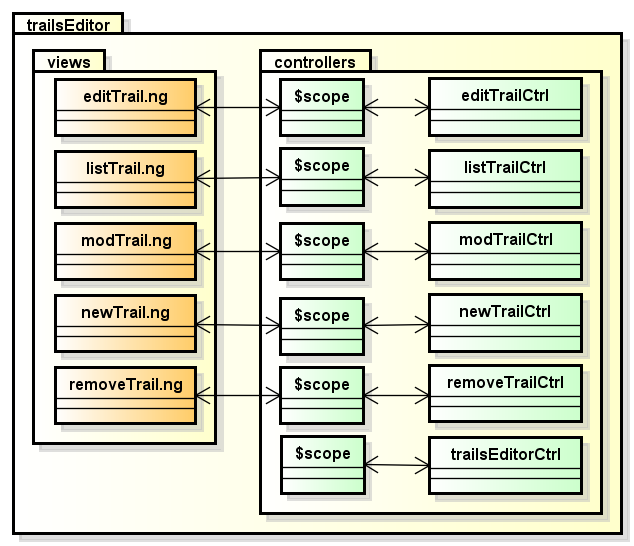
\includegraphics[scale=0.90]{img/diapkg/trailsEditor.png}
\caption{Diagramma del package premi/client/trailsEditor}
\end{center}
\end{figure}

%-------  diagramma di un template %
\subsubsection{premi/client/trailsEditor/views/basicToolbar.ng}

\begin{description}
%-------  descrizione del template%
\item[Descrizione] \hfill \\
	Template della vista associata allo \textit{\$scope} di \textit{basicToolbarCtrl}. Fornisce una toolbar per la navigazione tra le varie fasi della modifica della presentazione
\item[Note] \hfill \\
	\begin{itemize}
			\item Deve possedere un bottone per ogni fase dell'editor (Gestione Frame, Gestione Infografica e Gestione Trail)
			\item Deve possedere un bottone per l'uscita dall'editor
	\end{itemize}
\end{description}

%-------  diagramma di un template %
\subsubsection{premi/client/trailsEditor/views/editTrail.ng}

\begin{description}
%-------  descrizione del template%
\item[Descrizione] \hfill \\
	Template della vista associata allo \textit{\$scope} di \textit{editTrailCtrl}. Permette la modifica del titolo del trail selezionato dall'utente
\item[Note] \hfill \\
	\begin{itemize}
			\item Mostra il titolo del trail in un input HTML$_G$, modificabile, attraverso l'attributo dello scope \textit{Trail.title}
			\item Possiede un bottone associato al metodo \textit{save()} dello \textit{\$scope} per salvare le modifiche apportate al Trail
			\item Possiede un bottone associato al metodo \textit{discard()} dello \textit{\$scope} per annullare le modifiche effettuate sul trail
	\end{itemize}
\end{description}


%-------  diagramma di un template %
\subsubsection{premi/client/trailsEditor/views/listTrail.ng}

\begin{description}
%-------  descrizione del template%
\item[Descrizione] \hfill \\
	Template della vista associata allo \textit{\$scope} di \textit{listTrailCtrl}. Mostra la lista dei percorsi creati finora dall'utente associati alla presentazione
\item[Note] \hfill \\
	\begin{itemize}
			\item mostra una lista di tutti i percorsi attraverso l'attributo dello scope \textit{Trails}
			\item mostra una lista di tutti i frame inseribili attraverso il metodo dello scope \textit{getFramesId()}
	\end{itemize}
\end{description}

%-------  diagramma di un template %
\subsubsection{premi/client/trailsEditor/views/modTrail.ng}

\begin{description}
%-------  descrizione del template%
\item[Descrizione] \hfill \\
	Template della vista associata allo \textit{\$scope} di \textit{modTrailCtrl}. Deve consentire la modifica di un percorso in tutti i suoi attributi:
	\begin{itemize}
			\item inserimento di un frame in qualsiasi punto del percorso
			\item inserimento dello stesso frame più volte nel percorso
						\item spostamento di un frame da un punto all'altro del percorso
			\item eliminazione di un frame dal percorso
			\item trasformazione del frame in checkpoint
			\item elimiazione di un checkpoint
	\end{itemize}
\end{description}

%-------  diagramma di un template %
\subsubsection{premi/client/trailsEditor/views/newTrail.ng}

\begin{description}
%-------  descrizione del template%
\item[Descrizione] \hfill \\
	Template della vista associata allo \textit{\$scope} di \textit{newTrailCtrl}. Fornisce all'utente i comandi per l'inserimento di un novo trail associato alla presentazione nel database
\item[Note] \hfill \\
	\begin{itemize}
			\item Mostra un input HTML$_G$ associato all'attributo dello scope \textit{title} per l'inserimento del titolo del trail
			\item Possiede un bottone associato al metodo \textit{save()} dello \textit{\$scope} per salvare il nuovo Trail nel database
			\item Possiede un bottone associato al metodo \textit{discard()} dello \textit{\$scope} per annullare il processo di creazione del trail
	\end{itemize}
\end{description}

%-------  diagramma di un template %
\subsubsection{premi/client/trailsEditor/views/removeTrail.ng}

\begin{description}
%-------  descrizione del template%
\item[Descrizione] \hfill \\
	Template della vista associata allo \textit{\$scope} di \textit{removeTrailCtrl}. Fornisce all'utente i comandi per la rimozione di un trail associato alla presentazione dal database
\item[Note] \hfill \\
	\begin{itemize}
			\item Mostra un messaggio di conferma eliminazione del trail
			\item Possiede un bottone associato al metodo \textit{remove()} dello \textit{\$scope} confermare la rimozione
			\item Possiede un bottone associato al metodo \textit{discard()} dello \textit{\$scope} per annullare il processo di rimozione del trail
	\end{itemize}
\end{description}